\section{Software Verification}

Software programs are becoming increasingly complex. 
With the rise in complexity and technological advancements, components within a software have become susceptible to various erroneous conditions. 
Software verification have been perceived as a solution for the problems arising in the software development cycle. 
Software verification is primarily verifying if the specifications are met by the software\cite{ghezzi2002fundamentals}.

There are two fundamental approaches used in software verification - dynamic and static software verification\cite{ghezzi2002fundamentals}. 
Dynamic software verification is performed in conjunction with the execution of the software. 
In this approach, the behavior of the execution program is checked- commonly known as Test phase. 
Verification is succeeding phase also known as Review phase. 
In dynamic verification, the verification adheres the concept of test and experimentation. 
The verification process handles the test and behavior of the program under different execution conditions. 
Static software verification is the complete opposite of the previous approach. 
The verification process is handled by checking the source code of the program before its execution. 
Static code analysis is one such technique which uses a similar approach. 

The verification of software can also be classified in perspective of automation - manual verification and automated verification. 
In manual verification, a reviewer manually verifies the software. 
Whereas in the latter approach, a script or a framework performs  verification. 

Software verification is a very broad area of research. 
This thesis work is focussed on automated software verification for multithreaded programming. 

\section{Multithreaded Programming}

Computing power has grown over the years. 
Advancements are made in the domain of computer architecture by moving the computing power from single-core to multi-core architecture. 
With such advancement, there were needs to adapt the programming designs from a serialized execution to more parallelizable execution. 
Various parallel programming models were perceived to accommodate the perceived progression. 
Multithreaded programming model was one of the designs considered for the performance boost in computing\cite{carver2005modern}. 

Threads are a small tasks executed by a scheduler on an operating system, where the resources such as the processor, TLB (Translation Lookaside Buffer), cache, etc., are shared between them. 
Threads share the same address space and resources. 
Multithreading addresses the concept of using multiple threads for having concurrent execution of a program on a single or multi-core architectures. 
Inter-thread communication is achieved by shared memory. 
Mapping the threads to the processor core is done by the operating system scheduler. 
Multithreading is only supported in operating systems which has multitasking feature. 

Advantages of using multithreading include: 
\begin{itemize}
\item	Fast Execution
\item	Better system utilization
\item	Simplified sharing  and communication
\item 	Improved responsiveness - Threads can overlap I/O and computation.
\item	Parallelization
\end{itemize}

Disadvantages:
\begin{itemize}
\item	Race conditions
\item	Deadlocks with improper use of locks/synchronization
\item	Cache misses when sharing memory
\end{itemize}

\section{Concurrency Bugs}

Concurrency bugs are one of major concerns in the domain of multithreaded environment. 
These bugs are very hard to find and reproduce. 
Most of these bugs are propagated from mistakes made by the programmer\cite{lopez2017study}. 
Some of these concurrency bugs include:
\begin{itemize}
\item	Data Race
\item 	Order violation
\item	Deadlock
\item	Livelock
\end{itemize}

Non-deterministic execution behavior of threads is one of the reasons for having the among mentioned bugs. 
Data race and order violation are classified as race condition bugs. 
Whereas deadlock and livelock are classified as lack of progress bugs. 

\subsection{Race Condition}

Race condition is one of the most common concurrency problems.  
The problem arises when there are concurrent reads and writes of a shared memory location. 
As stated above, the problem occurs with non-deterministic execution behavior of threads. 

Consider the following example, where you have three threads and they share two variables x and y \cite{carver2005modern}. 
The value of x is initially 0. 

\begin{table}[h]
\centering
\begin{tabular}{*{3}{c}}
Thread 1 & Thread 2 & Thread 3 \\
\hline
 (1) x = 1 & (2) x = 2 & (3) y = x\\
\end{tabular}
\caption{Race condition example}
\label{race_cond}
\end{table}

If the statements (1), (2) and (3) were executed as a sequential program. 
The value of y would be 2. 
When the same program is split to three threads as shown in the above Table~\ref{race_cond}, the output of y becomes unpredictable. 
The possible values of y = {0,1,2}. 
The non-deterministic execution of the threads makes the output of y non-deterministic. 
Table~\ref{poss_exec} depicts possible executions for the above multithreaded execution. 

\begin{table}[h]
\centering
\begin{tabular}{*{2}{c}}
Execution Order & Value of y \\
\hline
 (3),(1),(2)& 0\\
 (3),(2),(1)& 0\\
 (2),(1),(3)& 1\\
 (1),(3),(2)& 1\\
 (1),(2),(3)& 2\\
 (2),(3),(1)& 2\\
\end{tabular}
\caption{Possible executions}
\label{poss_exec}
\end{table}

The above showcased problem is classified as race condition bug. 
Ordered execution of reads and writes can fix the problem. 

\subsection{Lack Of Progress}

Lack of progress is another bug class observed in multithreaded programs. 
Some of the bugs under this class include deadlocks and livelocks. 

\subsubsection{Deadlock}

Deadlock is a state in which each thread in thread pool is waiting for some other thread to take action. 
In terms of multithreaded programming environment, deadlocks occur when one thread waits on a resource locked by another thread, which in turn is waiting for another resource locked by another thread. 
If a thread is unable to change its state indefinitely because the resource requested by it are being held by another thread, then the entire system is said to be in deadlock. 

%----Example Picture depicting deadlock---
\tikzstyle{thread} = [circle, minimum size=.5cm, text centered, draw=black, fill=white!30]
\tikzstyle{resource} = [rectangle, minimum width=1cm, minimum height=1cm, text centered, draw=black, fill=white!30]

\begin{figure}[h]
\centering
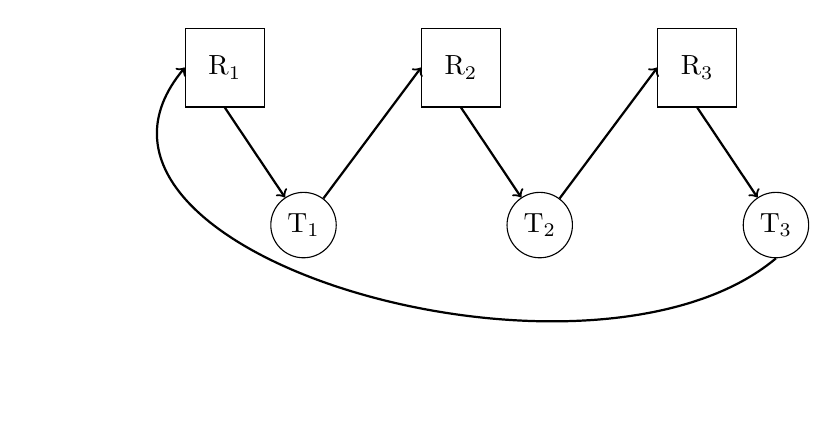
\begin{tikzpicture}[node distance=2cm]
%Resources
\node (R1) [resource] {R$_1$};
\node (R2) [resource,right of=R1,xshift =1cm] {R$_2$};
\node (R3) [resource,right of=R2,xshift =1cm] {R$_3$};

%Threads
\node (T1) [thread,below of=R1,xshift =1cm] {T$_1$};
\node (T2) [thread,below of=R2,xshift =1cm] {T$_2$};
\node (T3) [thread,below of=R3,xshift =1cm] {T$_3$};

%Arrows
\draw [->,thick] (R1.south) -- (T1);
\draw [->,thick] (R2.south) -- (T2);
\draw [->,thick] (R3.south) -- (T3);
\draw [->,thick] (T1) -- (R2.west);
\draw [->,thick] (T2) -- (R3.west);
\draw [->,thick] (T3.south) to [out=220,in=230] (R1.west);

\end{tikzpicture}
\caption{Dead Lock Example}
\label{deadlock_example}
\end{figure}

In the example depicted in Fig~\ref{deadlock_example}, we have three threads T$_1$, T$_2$,T$_3$ and three resource instances R$_1$, R$_2$, R$_3$. 
The figure depicts hold and wait by each threads. 
Thread T$_1$ holds resource R$_1$ and waits for the acquistion of resource R$_2$ from thread T$_2$. 
T$_2$ cannot relinquish resource R$_2$, unless it acquires resource R$_3$ for its progress. 
But, resource R$_3$ is acquired by T$_3$ and is waiting for R$_1$ from T$_1$. 
Thus, making a circular wait of resources. 
This example clearly explains the dependency of resources for the respective thread progress. 

Deadlock can occur if all the following conditions are met simultaneously.

\begin{itemize}
\item	Mutual exclusion
\item	Hold and wait
\item	No preemption
\item	Circular wait
\end{itemize}

These conditions are known as Coffman conditions.


\subsubsection{Livelock}

Livelock is similar to deadlock, except the state of threads change constantly but with none progressing. 

%\subsubsection{Partial Order Reduction}
%\subsubsection{Lipton}
%\subsubsection{Dynamic POR}

%\section{Model Checking}
%\section{Symbolic Execution}

%\section{Iterative Relaxed Scheduling}
%\section{Deterministic Multi-Threading}
